% LCFM @ NeurIPS 2026 — Workshop on Long Context Foundation Models
% Double-blind submission (author block omitted; provenance deferred to acceptance).
%
% Build: cd manuscript/workshop && tectonic main.tex
%
% Page budget: <= 8 pages of body (references excluded), per the LCFM CFP
% (long-paper option). Style: official NeurIPS 2026 package (dblblindworkshop).

\documentclass{article}

\usepackage[dblblindworkshop]{neurips_2026}
\workshoptitle{Workshop on Long Context Foundation Models (LCFM) @ NeurIPS 2026}

\usepackage[utf8]{inputenc}
\usepackage[T1]{fontenc}
\usepackage[hidelinks]{hyperref}
\usepackage{url}
\usepackage{booktabs}
\usepackage{amsfonts}
\usepackage{amsmath}
\usepackage{amssymb}
\usepackage{textcomp}
\usepackage{microtype}
\usepackage{xcolor}
\usepackage{graphicx}
\usepackage{enumitem}

\graphicspath{{../../figures/}{./}}

\urlstyle{tt}
\Urlmuskip=0mu plus 1mu
\emergencystretch=3em

% Double-blind: no author block. The block is restored on acceptance.
\author{}

\title{When Speculative Decoding Stops Paying Off at Long Context:\\
       A Diagnostic Study with RASD}

\begin{document}
\maketitle

% =========================================================================
\begin{abstract}
Speculative decoding's 2--3$\times$ short-context speedups do not
reliably transfer to million-token inference. This paper asks \emph{when and
why the transfer stops}. On Llama-2-7B extended to 1\,M tokens with
YaRN factor 256, per-round acceptance becomes bimodal: across the
measured long contexts, 48\% of verify rounds fully reject the draft
(pooled Wilson 95\% CI $[0.39, 0.57]$) and the median per-round
$\alpha$ is exactly 0 at 128\,k and 512\,k. The paired per-seed
speedup against a matched target-only baseline regresses from
$1.76\times$ $[1.59, 1.93]$ at 256\,k to $0.94\times$ $[0.57, 1.30]$
at 512\,k and $0.97\times$ $[0.80, 1.14]$ at 1\,M, statistical
parity. A PG-19 dose-response ($\alpha$: $0.71$@4\,k $\to$ $0.26$@8\,k $\to$
$0.11$@1\,M) supports context length as the primary driver. A profiler measurement shows communication is
${\leq}1.2\%$ of wall on the speculator rank, ruling out
communication-overlap masking. The measured speedup is instead set
by a race between two mechanisms: the acceptance collapse, and the
growing cost of the speculative round itself (\S\ref{sec:speedup}).
Arriving at these
findings required a system that runs a target-model forward at
1\,M context: \textbf{RASD} combines ring-attention sequence
parallelism, NF4 KV-cache quantization, YaRN scaling, and
speculative verification, and reaches 1\,M tokens at 39.3\,GiB peak
per rank on 8$\times$A100, where the vanilla HuggingFace
FlashAttention-2 stack OOMs at 128\,k. Code, traces, and the
ablation grid will be released upon acceptance.
\end{abstract}

% =========================================================================
\section{Introduction}
\label{sec:intro}

Speculative decoding \citep{leviathan2023fast,chen2023accelerating}
is the standard technique for amortizing autoregressive LLM
decoding: a small draft model proposes $\gamma$ tokens and the
target model verifies them in one forward pass, accepting the
longest matching prefix. At short context it routinely yields
$2$--$4\times$ wall-clock speedups with provably identical output
distributions, and its behavior in that regime is well understood.
Its behavior at \emph{long} context, the regime where
long-context foundation models, agentic trace accumulation, and
repository-scale inference actually operate, is essentially
unmeasured. Prior speculative-decoding systems evaluate at
short-to-moderate context
\citep{miao2023specinfer,cai2024medusa,li2024eagle}; their
acceptance rates at $10^5$--$10^6$ tokens are unknown.

The question this paper asks is deliberately narrow and
diagnostic: \emph{at what context length does speculative decoding
stop paying off, and what mechanism makes it stop?} Answering it
requires a system that can run a target-model forward at 1\,M
context on commodity hardware. We built such a system,
\textbf{RASD} (ring attention with speculative decoding), but the
system is the \emph{vehicle} for the measurement, not the
contribution. The contribution is a set of findings about the
regime in which speculation is useful, three of which follow.

\textbf{Finding 1 (acceptance becomes bimodal).} At every long
context we measure (128\,k--1\,M), roughly half of all verify
rounds fully reject the draft ($\alpha = 0$), and most remaining
rounds accept 1--2 of the 4 proposed tokens, with a small tail of
fuller acceptances. The median per-round
$\alpha$ is exactly 0 at 128\,k and 512\,k. The 3-seed matrix
mean acceptance is 0.090 / 0.201 / 0.172 / 0.178 at
128\,k / 256\,k / 512\,k / 1\,M: non-monotone in context, so
acceptance alone cannot explain the speedup shape
(\S\ref{sec:speedup}). The aggregate means hide a two-mode
distribution, not a unimodal distribution around the mean
(\S\ref{sec:bimodal}).

\textbf{Finding 2 (context length, not prompt source, is the
primary driver).} A dose-response on real text (PG-19) shows mean
acceptance decaying monotonically with context
($\alpha = 0.71$@4\,k, $0.26$@8\,k, $0.11$@1\,M), so the
collapse persists even when the synthetic prompt is replaced with
narrative text (\S\ref{sec:dose-response}).

\textbf{Finding 3 (communication overlap is not the mechanism).}
The original RASD design hypothesis was that the speculative draft
pass could hide ring-attention communication latency. A
torch.profiler measurement shows communication is $\leq 1.2\%$ of
wall on the speculator rank at $W=8$ over NVLink; the overlap
budget does not exist at this scale. The measured speedup is set
by a race between two other mechanisms: the acceptance collapse
and the growing cost of the speculative round itself
(\S\ref{sec:speedup}).

\textbf{The headline consequence.} The paired per-seed speedup of
RASD against a matched target-only baseline (identical
infrastructure, speculative loop disabled) is
$1.27\times$ $[0.80, 1.74]$ at 128\,k,
$1.76\times$ $[1.59, 1.93]$ at 256\,k, then regresses to
$0.94\times$ $[0.57, 1.30]$ at 512\,k and
$0.97\times$ $[0.80, 1.14]$ at 1\,M
(\S\ref{sec:speedup}). At the headline scale, speculative decoding
adds nothing; we own and quantify that rather than obscure it.

Two scope notes. First, these findings are measured on
Llama-2-7B \citep{touvron2023llama2} under YaRN
\citep{peng2023yarn} factor 256, a configuration whose base model
is far out of distribution beyond its 4\,k training context. That
is a \emph{deliberate} worst-case probe, not an oversight
(\S\ref{sec:limitations}): it exposes the OOD acceptance collapse
in its strongest form, and it is the regime a long-context base
model would encounter more gradually. Second, RASD's capability
claim (1\,M-token inference at 39.3\,GiB/rank) is real but
secondary here; we report it in one section
(\S\ref{sec:capability}) and otherwise treat the system as
measurement infrastructure.

% =========================================================================
\section{Background and Related Work}
\label{sec:related}

\textbf{Long-context inference.} Ring attention
\citep{liu2023ringattention} shards the sequence across devices and
pipelines attention through a ring of KV exchanges, making
per-device memory $\mathcal{O}(N/W)$ and exact. FlashAttention
\citep{dao2022flashattention,dao2023flashattention2} supplies the
IO-aware local kernel; FlashDecoding
\citep{dao2023flashdecoding} parallelizes single-query decode
attention intra-rank. KV quantization (NF4
\citep{dettmers2023qlora,dettmers2022bitsandbytes}, KIVI
\citep{liu2024kivi}, KVQuant \citep{hooper2024kvquant})
compresses the cache; vLLM \citep{kwon2023vllm} manages it in
paged blocks. Attention-sink prefixes \citep{xiao2024streamingllm}
and position scaling (YaRN \citep{peng2023yarn}, LongRoPE-style
frequency search) extend short-context base models; architectural
alternatives such as StripedHyena \citep{poli2023stripedhyena}
and MInference \citep{jiang2024minference} avoid or sparse the
attention cost entirely. RASD composes ring attention, NF4 KV
quantization, YaRN, and attention sinks; none of these prior
systems reports speculative-acceptance behavior at 1\,M context.

\textbf{Speculative decoding.} \citet{leviathan2023fast} and
\citet{chen2023accelerating} introduced draft-verify decoding with
a provably distribution-preserving acceptance rule; expected
tokens per target call is
\begin{equation}
\label{eq:spec-tokens}
\mathbb{E}[\text{tokens}] = \frac{1 - \alpha^{\gamma+1}}{1 - \alpha},
\end{equation}
so throughput depends on $\alpha$ and on the cost of the
speculative round itself (\S\ref{sec:speedup}).
Eq.~\ref{eq:spec-tokens} is the i.i.d. idealization, in which
each rejection restarts a fresh geometric trial. The standard
residual-resampling acceptance rule used in implementations emits
at least one token per round regardless of rejection, so the
measured tokens per round is approximately $1 + \gamma \bar\alpha$,
and Eq.~\ref{eq:spec-tokens} understates it (\S\ref{sec:speedup}).
Throughout, our measured $\alpha$ is the per-round
accepted-token fraction (accepted tokens divided by drafted
tokens), not the i.i.d. per-token acceptance parameter assumed by
Eq.~\ref{eq:spec-tokens}; the two coincide only under the
equation's independence assumptions.
Medusa \citep{cai2024medusa} and EAGLE
\citep{li2024eagle} replaced the separate draft model with heads
on the target; EAGLE-2/3 improved draft trees further. All report
acceptance at short-to-moderate context. The natural mechanism
question at long context is therefore: \emph{does $\alpha$ itself
collapse?} This paper measures it.

\textbf{The overlap hypothesis.} In distributed decode, each
round pays a communication cost $\delta_{\text{comm}}$ for the KV
rotation. Because a draft pass needs only the current KV state, it
can in principle run on a separate CUDA stream while the target
waits for the next block, hiding $\delta_{\text{comm}}$ entirely.
This predicted an \emph{additive} speedup beyond
Eq.~\ref{eq:spec-tokens}. \S\ref{sec:comm} tests this hypothesis
and rejects it at our scale, a negative result with practical
value for anyone designing distributed speculative systems.

% =========================================================================
\section{The RASD System}
\label{sec:system}

RASD (Ring Attention with Speculative Decoding) is a decode loop
on $W=8$ A100 80\,GB SXM4 GPUs (NVLink-interconnected, single
node). Both the target model (Llama-2-7B) and a draft model
(Sheared-LLaMA-1.3B \citep{xia2023sheared}, which shares the
target's tokenizer) are loaded on every rank with NF4-quantized
weights. The draft is deliberately not YaRN-extended: it retains
its native 4\,k position cap and attends over only the most
recent 4{,}096 tokens of the sequence (its KV cache covers that
truncated window and is kept in bf16), while its weights are
NF4-quantized like the target's. The draft's forward cost is
therefore nearly context-independent, which matters for the
mechanism analysis in \S\ref{sec:speedup}. One decode round proceeds as follows: \textbf{(1)} the
draft proposes $\gamma=4$ tokens autoregressively on all ranks;
\textbf{(2)} the target verifies the $\gamma+1$ positions in a
single packed forward over ring attention, with FlashAttention-2
inside each local block and KV blocks rotating via
\texttt{batch\_isend\_irecv}; \textbf{(3)} draft and target logits
are broadcast from rank 0; \textbf{(4)} every rank runs the
acceptance test $\min(1, p_{\mathrm{target}}/p_{\mathrm{draft}})$
and resamples rejected positions from
$\max(0, p-q)/Z$ \citep{leviathan2023fast}, using a shared RNG seed
so KV updates are bit-identical across ranks.

The memory configuration that fits 1\,M context: K and V are
NF4-quantized with a chunked update path (transient under
100\,MiB), a bf16 attention-sink prefix of the first 128 tokens
\citep{xiao2024streamingllm} is held on rank 0 only, and position
embeddings use YaRN with $f = \lceil N/4096 \rceil$ ($f=256$ at
1\,M). Per-rank peak memory is dominated by weights (${\approx}4$
GiB) plus the NF4 KV shard $\tfrac{N}{W} L\, 2 d_h \tfrac{1}{2}$;
measured peaks run ${\approx}15$ GiB above this sketch at 1\,M due
to transient and scratch buffers. The full memory derivation
appears in the extended version (anonymized supplementary).

The design point ($\gamma=4$, KV block size $c=2048$, Sheared
draft, prefetch depth 1) was fixed by the M3 ablation grid, five
one-factor-at-a-time sweeps at 64\,k context with 3 seeds each.
The dominant lever is block size: throughput rises
$0.62 \to 0.87 \to 1.11 \to 1.25$ tok/s across
$c \in \{256, 512, 1024, 2048\}$, a $2\times$ improvement, at
unchanged acceptance (0.253). The other four axes fix smaller
knobs; the full 49-row grid ships with the artifact release.

\textbf{Baseline.} Every speedup in this paper is against the
\emph{target-only} configuration: the identical RASD loop with
$\gamma=0$ (no draft model, no verify). Ring attention, NF4 KV,
YaRN, and the sink prefix are identical; exactly one variable,
the speculative loop, differs. This isolates the speculative
mechanism from the distributed-KV infrastructure.

% =========================================================================
\section{Measurement Setup}
\label{sec:setup}

\textbf{Main matrix.} Four contexts
$\{128, 256, 512, 1024\}$\,k $\times$ three seeds
$\{42, 123, 456\}$, for both RASD and target-only, with a
controlled synthetic-fill protocol (a deterministic
repeated-paragraph prompt that fills the context window,
isolating system behavior from prompt-content variance). Each run
reports throughput, mean acceptance, latency, and per-rank peak
memory.

Each run targets 64 new tokens (the cap is checked before each
round, so the final speculative round may overshoot by up to
$\gamma$ tokens; some cells log 65--66) and stops early at the
first EOS token. In the degenerate YaRN regime the 128\,k spec
cells (and one target-only seed) terminated on EOS after 16--27
tokens, versus 64--66 elsewhere. Throughput and \texttt{time\_sec}
include prefill (TTFT is recorded separately). Recomputing the
128\,k paired ratio on decode-only time,
$(\texttt{time\_sec} - \texttt{ttft\_ms}/1000)/\texttt{tokens}$,
gives a paired mean of $1.44\times$ $[0.76, 2.12]$ instead of
$1.27\times$; at 256\,k and above the convention shifts the ratio
by at most $0.11\times$. The early-EOS length mismatch biases only
the 128\,k cell; Table~\ref{tab:speedup} reports the inclusive
convention, matching the logged throughput.

\textbf{Per-round traces.} For the seed-42 run at each long
context we logged one JSONL sidecar per verify round (round index,
position, draft tokens, accepted count), the source of the
exact acceptance distributions in \S\ref{sec:bimodal}.

\textbf{PG-19 control.} Single-seed (42) runs on PG-19 narrative
text \citep{rae2019pg19} at 4\,k and 8\,k (both spec and
target-only) and at 1\,M (spec only), the dose-response in
\S\ref{sec:dose-response}.

\textbf{Profiler subset.} torch.profiler captures at
$\{32, 128, 256, 512\}$\,k (single seed), bucketed into compute /
comm / idle / other on rank 0. The 1\,M profiler cell did not
complete; see \S\ref{sec:limitations}.

\textbf{Reproducibility.} All package versions are pinned in a
lockfile; every number in this paper is a commit of a CSV or JSONL
sidecar. Code, the lockfile, traces, and the W\&B run IDs are
released upon acceptance.

% =========================================================================
\section{Findings}
\label{sec:findings}

\subsection{Per-round acceptance is bimodal at long context}
\label{sec:bimodal}

Figure~\ref{fig:bimodality} and Table~\ref{tab:distribution}
report the per-round acceptance structure at the four long
contexts, from the seed-42 traces. The aggregate means
(11.5--21.3\% for the seed-42 trace) are not
unimodal-around-the-mean: at every context, roughly half of rounds
fully reject the draft, and most remaining rounds accept 1--2 of
the 4 proposed tokens, with a tail of fuller acceptances at
256\,k (three rounds accept all four tokens) and 512\,k (one
round accepts three). The median per-round $\alpha$ is
exactly 0 at 128\,k and 512\,k. Pooling all long-context rounds
($n=119$), $P(\alpha{=}0) = 57/119 = 0.48$ (Wilson 95\% CI
$[0.39, 0.57]$). Per-context $P(\alpha{=}0)$, again Wilson 95\%:
0.54 $[0.27, 0.81]$ at 128\,k, 0.47 $[0.30, 0.64]$ at 256\,k,
0.53 $[0.36, 0.69]$ at 512\,k, and 0.42 $[0.26, 0.58]$ at 1\,M.
We report the exact discrete distribution and a binomial CI on
$P(\alpha{=}0)$ rather than a dip test: with 13--36 rounds per
context, a dip statistic would be noise.

\begin{figure}[t]
\centering
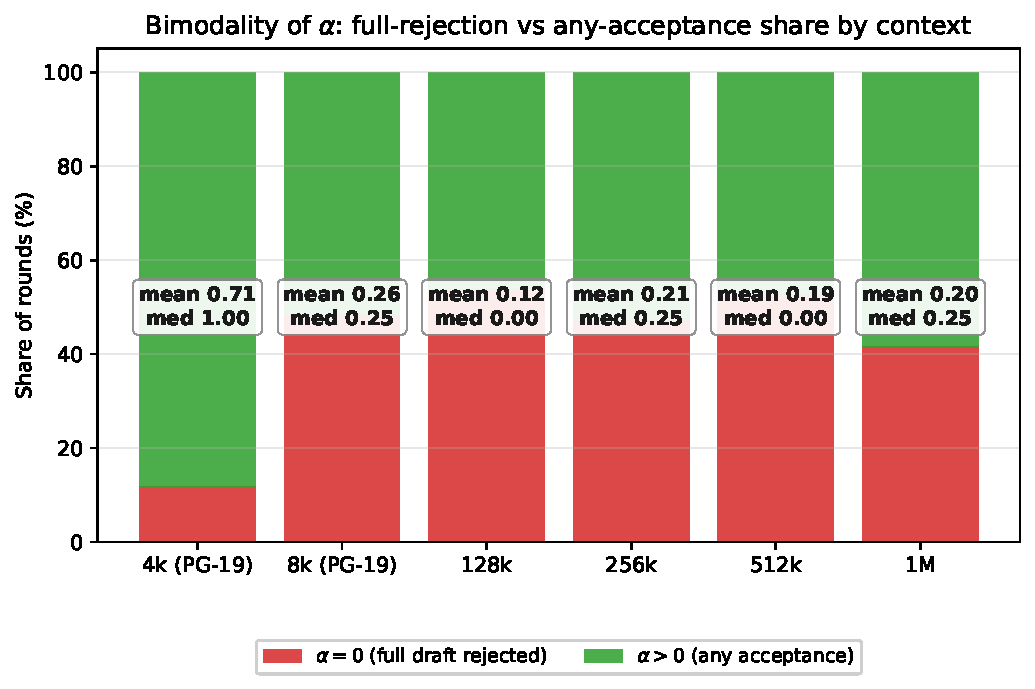
\includegraphics[width=0.78\linewidth]{fig4b_bimodality.pdf}
\caption{Per-context share of verify rounds that fully reject the
draft ($\alpha = 0$) vs.\ accept at least one token ($\alpha > 0$),
seed-42 traces. Annotations report mean and median $\alpha$. At
every long context roughly half of rounds fully reject the draft.}
\label{fig:bimodality}
\end{figure}

\begin{table}[t]
\centering
\footnotesize
\caption{Exact counts of verify rounds by number of accepted draft
tokens (of $\gamma=4$), synthetic prompts, seed-42 traces.
Columns 0/1/2/$\ge$3 are accepted-token counts (a round accepting
$k$ tokens has $\alpha = k/4$); e.g., at 512\,k the mean is
$(7\cdot1 + 9\cdot2 + 1\cdot3)/36$ tokens per round, i.e.,
$\alpha = 0.194$.}
\label{tab:distribution}
\begin{tabular}{lrrrrrrr}
\toprule
Context & rounds & 0 & 1 & 2 & $\ge$3 & mean $\alpha$ & median $\alpha$ \\
\midrule
128\,k & 13 & 7  & 6 & 0 & 0 & 0.115 & 0 \\
256\,k & 34 & 16 & 13 & 2 & 3 & 0.213 & 0.25 \\
512\,k & 36 & 19 & 7  & 9 & 1 & 0.194 & 0 \\
1\,M   & 36 & 15 & 13 & 8 & 0 & 0.201 & 0.25 \\
\bottomrule
\end{tabular}
\end{table}

\textbf{Mechanism.} In the YaRN-extrapolated regime the target's
logits are near-uniform over a large effective vocabulary (PPL
$=814$ at 32\,k under YaRN factor 8, versus ${\approx}12$ at
native 4\,k). A 1.3B draft cannot reduce that entropy: each draft
token carries probability ${\sim}10^{-3}$ under the target, so
verify rejects all four. On the rounds where the target does
commit to a high-probability continuation, the draft tracks and
1--2 (occasionally all four) tokens are accepted. The bimodality
is therefore consistent with target-logit entropy, not a defect of
the verify loop: at native
4\,k the same system concentrates near $\alpha = 1$
(\S\ref{sec:dose-response}).

\subsection{Context length, not prompt source, is the primary driver}
\label{sec:dose-response}

A competing explanation for the collapse is the \emph{synthetic
prompt}: repeated-paragraph prompts carry no semantic momentum, so
low acceptance could be a prompt artifact rather than an OOD
artifact. Table~\ref{tab:pg19} reports a dose-response on PG-19
narrative text. Mean $\alpha$ decays monotonically
($0.71$@4\,k, $0.26$@8\,k, $0.11$@1\,M), and the bimodality
appears by 8\,k on real text ($P(\alpha{=}0) = 15/31$), even
though 8\,k is only $2\times$ the model's 4\,k training window.
Critically, at 1\,M \emph{real} text, acceptance falls to 0.108,
at or below the synthetic-prompt 1\,M value (0.201, seed 42). If
the synthetic prompt were the driver, PG-19 at 1\,M should recover
native-context acceptance; it does not. The dose-response supports
context length (base-model OOD under YaRN extrapolation) as the
primary driver, with prompt source a secondary
modifier. All rows are a single seed (42), an acknowledged
limitation (\S\ref{sec:limitations}).

\begin{table}[t]
\centering
\footnotesize
\caption{PG-19 dose-response (seed 42, one seed per row). Speedup
is spec vs.\ target-only on the same prompt at the same context;
no target-only 1\,M PG-19 run exists. $^{\dagger}$No per-round
trace was saved for the 1\,M PG-19 run; median and
$P(\alpha{=}0)$ are unavailable.}
\label{tab:pg19}
\begin{tabular}{lrrrrr}
\toprule
Context & mean $\alpha$ & median $\alpha$ & $P(\alpha{=}0)$ & rounds & speedup \\
\midrule
4\,k & 0.706 & 1.0   & $2/17$ & 17 & $4.4\times$ \\
8\,k & 0.258 & 0.25  & $15/31$ & 31 & $2.3\times$ \\
1\,M & 0.108 & n/a$^{\dagger}$ & n/a$^{\dagger}$ & 44 & n/a \\
\bottomrule
\end{tabular}
\end{table}

\subsection{Paired speedup regresses to parity}
\label{sec:speedup}

Table~\ref{tab:speedup} reports per-seed speedup ratios
$\mathrm{RASD}_i / \mathrm{target}_i$ for matched seeds, with
$t$-based 95\% CIs on the ratio ($df=2$), tighter and more
honest than marginal CIs on throughput. The shape is
non-monotonic: a large and significant speedup at 256\,k
($1.76\times$), then a point-estimate \emph{regression} at 512\,k
($0.94\times$) and parity at 1\,M ($0.97\times$). The 128\,k and
512\,k intervals straddle 1, reflecting three-seed noise on
multi-hour runs; the 256\,k interval excludes 1. Figure~\ref{fig:throughput}
plots the underlying throughputs, including the vanilla
HuggingFace FlashAttention-2 ceiling (OOM at $\geq$128\,k
single-rank).

\begin{table}[t]
\centering
\footnotesize
\caption{Per-seed paired speedup ratios
$\mathrm{RASD}_i / \mathrm{target}_i$ at matched context and seed,
the paired mean, and a $t$-based 95\% CI ($df=2$). The last two
columns decompose the seed-42 speedup: tokens per round (spec)
and the spec round cost relative to a target-only forward.
Speedup $=$ (tokens/round, spec $\div$ tokens/round, target-only)
$\times$ (target-only round cost $\div$ spec round cost); the
identity holds per seed. Target-only tokens/round is 1.02 in all
cells except the early-EOS 128\,k $s{=}456$ cell (1.05).
Three-seed means of the round-cost ratio: 1.11 (128\,k), 1.02
(256\,k), 1.79 (512\,k), 1.76 (1\,M); tokens/round: 1.43, 1.83,
1.71, 1.74. Mean throughputs (tok/s) for reference: RASD
$0.266 / 0.237 / 0.086 / 0.043$; target-only
$0.212 / 0.134 / 0.091 / 0.044$.}
\label{tab:speedup}
\begin{tabular}{lrrrrrrr}
\toprule
Context & $s{=}42$ & $s{=}123$ & $s{=}456$ & paired mean & 95\% CI & tokens/round & cost ratio \\
\midrule
128\,k & 1.33 & 1.42 & 1.06 & $1.27\times$ & $[0.80, 1.74]$ & 1.54 & 1.14 \\
256\,k & 1.82 & 1.78 & 1.69 & $1.76\times$ & $[1.59, 1.93]$ & 1.88 & 1.02 \\
512\,k & 0.97 & 1.07 & 0.78 & $0.94\times$ & $[0.57, 1.30]$ & 1.81 & 1.84 \\
1\,M   & 1.00 & 1.02 & 0.89 & $0.97\times$ & $[0.80, 1.14]$ & 1.83 & 1.81 \\
\bottomrule
\end{tabular}
\end{table}

\begin{figure}[t]
\centering
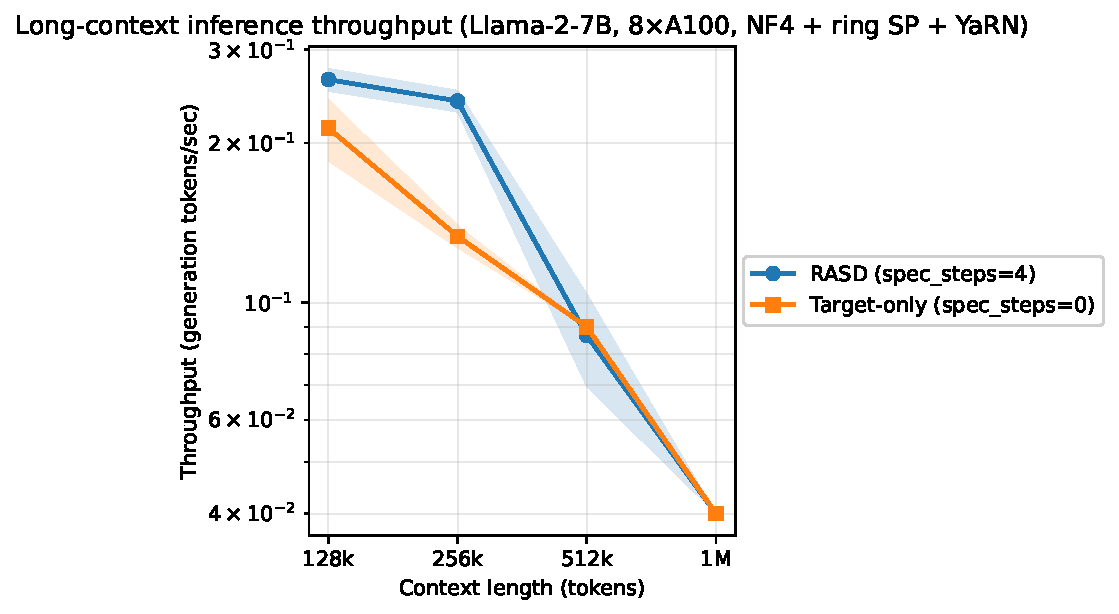
\includegraphics[width=0.72\linewidth]{fig1_throughput_vs_context.pdf}
\caption{Throughput vs.\ context. RASD (blue) and matched
target-only (orange) at 4 contexts $\times$ 3 seeds; vanilla HF
FA-2 \texttt{generate()} completes only at 32\,k (OOM markers at
$\geq$128\,k). Bands are 95\% CIs ($\pm 1.96$\,SEM) over seeds
for display; the paired ratio CIs in Table~\ref{tab:speedup} are
$t$-based.}
\label{fig:throughput}
\end{figure}

The honest reading: at the headline scale the speculative loop
adds nothing on this base model, and the interesting question is
where the payoff lives. The non-monotonic curve is a two-mechanism
story, and the speedup factorizes exactly: speedup $=$
(tokens/round, spec $\div$ tokens/round, target-only) $\times$
(target-only round cost $\div$ spec round cost), where tokens/round
$=$ \texttt{tokens\_generated}/\texttt{n\_rounds} and round cost
$=$ \texttt{time\_sec}/\texttt{n\_rounds}. \emph{Mechanism (a),
acceptance collapse}: $\alpha$ falls from 0.71 at 4\,k to the
0.09--0.20 band at long contexts, capping measured tokens/round at
1.43 (128\,k), 1.83 (256\,k), and 1.71--1.74 (512\,k--1\,M),
versus 3.9 at 4\,k. \emph{Mechanism (b), round-cost inflation}:
the spec round costs $1.02\times$ a target-only forward at 256\,k
but $1.79\times$ at 512\,k and $1.76\times$ at 1\,M. Mechanism
(b), not $\alpha$, produces the 256\,k$\to$512\,k cliff:
tokens/round barely moves ($1.83 \to 1.71$) while the round-cost
ratio nearly doubles, and flat $\alpha$ (0.201 / 0.172 / 0.178)
coexists with a swinging speedup (1.76 / 0.94 / 0.97). Which
component of the speculative round drives the inflation is not
isolated: the four draft passes are nearly context-independent by
construction (the draft window is capped at 4\,k,
\S\ref{sec:system}), so the packed five-position verify and its
per-round overheads are the leading candidates, hypothesis only.

Two accounting notes. First, the measured $1.76\times$ at 256\,k
exceeds the Eq.~\ref{eq:spec-tokens} ceiling at $\alpha \approx
0.20$ ($1.25\times$). The gap is the idealization gap: residual
resampling emits at least one token per round, and acceptance is
heterogeneous across rounds, so measured tokens/round ($1.83$)
exceeds the i.i.d. prediction. Per seed, the factorization above
reproduces the measured ratios exactly, leaving no residual; any
residual beyond the factorization would be an
infrastructure-level asymmetry that we do not isolate. Second, we
report measured tokens/round throughout and treat
Eq.~\ref{eq:spec-tokens} as the i.i.d. idealization only.

\subsection{Communication overlap is not the mechanism}
\label{sec:comm}

The original RASD hypothesis was that the speculative draft pass
hides ring-communication latency. We test it directly. Figure~\ref{fig:breakdown}
shows the rank-0 time-share buckets across contexts: \emph{comm}
(the sum of NCCL / c10d / \texttt{batch\_isend\_irecv} event
self-times, an \emph{issued} upper bound that includes the
tick-gate barrier and therefore upper-bounds the overlap-eligible
\emph{exposed} comm) is $1.0$--$1.2\%$ of wall at every context
(from the 32\,k canary through 512\,k). Rank-0 idle is ${\geq}50\%$
(synchronization covered by useful compute on the other seven
ranks). The overlap budget that motivated the design does not
exist at $W=8$ on NVLink: $\delta_{\text{comm}} \ll t_{\text{verify}}$.
Communication overlap is therefore not the mechanism behind any
speedup in this paper; the two-mechanism decomposition of
\S\ref{sec:speedup} (acceptance collapse versus round-cost
inflation) is. This is a
useful negative result: the ring-attention collective is already
communication-efficient at this scale, and distributed speculative
systems should not budget for overlap masking here. At $W \geq 32$
or over PCIe/InfiniBand the budget plausibly returns; we do not
test it.

\begin{figure}[t]
\centering
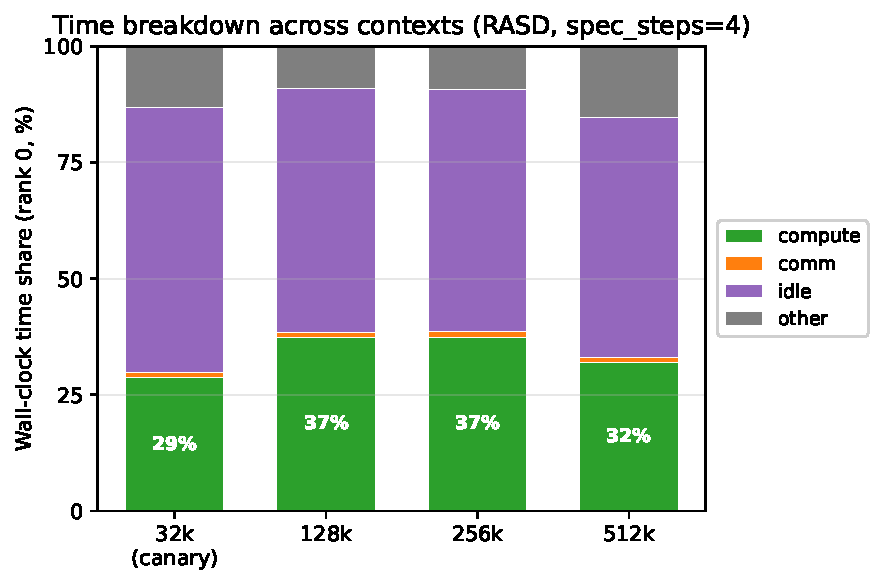
\includegraphics[width=0.62\linewidth]{fig3_time_breakdown.pdf}
\caption{Rank-0 time breakdown across contexts (profiler subset,
single seed). Comm is $\leq 1.2\%$ of wall at every context;
idle is the synchronization share covered by compute on other
ranks.}
\label{fig:breakdown}
\end{figure}

% =========================================================================
\section{Capability and Design Point}
\label{sec:capability}

One paragraph, because it is context for the findings rather than
the contribution. RASD reaches 1\,M-token Llama-2-7B inference at
39.3\,GiB peak per rank (8$\times$A100 80\,GB SXM4), $+0.9$\,GiB
over the target-only configuration at the same context, the
cost of the draft model and its KV cache. The vanilla HuggingFace
FlashAttention-2 \texttt{generate()} path OOMs during prefill at
every context $\geq$128\,k single-rank (bf16 KV cache alone is
${\approx}512$\,GiB at 1\,M), completing only the 32\,k cell
(30.1\,GiB, 7.25 tok/s). The combination of ring-attention
sharding and NF4 KV quantization is what fits the configuration;
the $2\times$ block-size lever from the M3 grid
(\S\ref{sec:system}) is the single most consequential engineering
choice, and the remaining four sweeps fix $\gamma=4$, the
Sheared-1.3B draft, and prefetch depth 1. The full grid and the
memory accounting ship with the artifact release.

% =========================================================================
\section{Limitations}
\label{sec:limitations}

\textbf{Parity at 1\,M is owned, not hidden.} The title of this
paper is the finding. At 1\,M the paired speedup is
$0.97\times$ $[0.80, 1.14]$, statistical parity, and at
512\,k the point estimate is a $0.94\times$ regression whose CI
straddles 1. We do not present these as wins.

\textbf{Llama-2's 4\,k window is a deliberate worst-case probe.}
A base model trained at 4\,k context and stretched by YaRN factor
256 is the strongest available OOD stress test of speculative
acceptance. A long-context base model would traverse the same OOD
gradient more gradually, and the dose-response
(\S\ref{sec:dose-response}) suggests the collapse point moves out
rather than disappearing. This is a hypothesis, not a
demonstration; the choice of base model is the reason every
finding in this paper is scoped to ``Llama-2-7B under YaRN.''

\textbf{Single-seed cells.} The PG-19 dose-response, the profiler
subset, and the per-round traces are single-seed (42). The
dose-response trend is monotone and large, but the $1.76\times$ at
256\,k is the only speedup whose CI excludes 1, and three seeds is
itself thin. Per-context $P(\alpha{=}0)$ CIs in
Table~\ref{tab:distribution} are wide by construction.

\textbf{Small-$n$ distributional claims.} The bimodality is
reported as an exact discrete distribution with a binomial CI on
$P(\alpha{=}0)$; with 13--36 rounds per context we deliberately
avoid distributional tests (e.g., dip statistics) that would not
be powered.

\textbf{An unruled-out mechanism.} The draft and target models
are independently NF4-quantized; divergence between their
independently quantized logits could contribute to rejection
rounds. The proposed isolation is a bf16 draft at 64\,k, deferred
to future work.

\textbf{No production-stack baseline.} We compare against a
matched target-only ablation and the vanilla HF FA-2 ceiling, not
vLLM / TensorRT-LLM at matched contexts; the target-only ablation
is the correct control for the speculative mechanism, but a
production-stack comparison at 128\,k--256\,k is a
follow-up.

\textbf{Scope of the comm result.} $\leq 1.2\%$ comm is measured
on rank 0 of one 8-GPU NVLink node. Non-rank-0 profiles and
multi-node configurations are unmeasured; the negative result is
scoped to $W=8$, NVLink, single node.

\textbf{Missing 1\,M profiler cell.} The torch.profiler
aggregation at 1\,M did not return within 2\,h of CPU work; the
profiler matrix stops at 512\,k, and the comm narrative
extrapolates the flat 32\,k--512\,k trend.

% =========================================================================
\section{Conclusion}
\label{sec:conclusion}

We asked when speculative decoding stops paying off at long
context, and measured the answer on a system built to ask the
question. On Llama-2-7B under YaRN factor 256: acceptance becomes
bimodal (half of rounds reject the draft entirely), the collapse
is driven by context length rather than prompt source, the paired
speedup regresses from $1.76\times$ at 256\,k to parity at 1\,M,
and communication overlap, the mechanism we originally designed
for, is absent at $W=8$ on NVLink, leaving the acceptance collapse
and the round-cost inflation of \S\ref{sec:speedup} as the
operative mechanisms. The practical message for
long-context serving is twofold: budget speculative decoding by
\emph{measured} acceptance and round cost in the deployed context
regime, not by short-context benchmarks; and on NVLink nodes, do
not expect the draft pass to buy communication hiding. RASD remains as the
measurement instrument: 1\,M-token inference at 39.3\,GiB/rank,
with every trace released upon acceptance so the community can
re-derive each claim.

% =========================================================================
% References (not counted in the 8-page budget)
% =========================================================================
\bibliographystyle{plainnat}
\bibliography{../bib/references}

\end{document}
